\documentclass[12pt]{beamer}
\usepackage{amsmath,amssymb,amsfonts,amsthm}
\beamertemplatefootpagenumber
\usepackage{threeparttable}
\geometry{paperwidth=150mm,paperheight=125mm}
\usepackage{lipsum}
\usepackage{ragged2e} % 文字向兩邊對齊
\useinnertheme{rectangles}  % change the theme

\usepackage{float}
\usepackage{multirow}
\usepackage{makecell}
\usepackage{siunitx}
%\usepackage{booktabs}

%打中文需要以下packages
\usepackage{xeCJK} 
\setCJKmainfont[BoldFont={cwTeXHeiBold}, ItalicFont={FandolSong}]{cwTeXMing} %Overleaf 中文字型設定
%\setCJKmainfont[BoldFont={cwTeX Q HeiZH}, ItalicFont={新細明體}]{cwTeX Q Ming}	
\XeTeXlinebreaklocale "zh"
\XeTeXlinebreakskip = 0pt plus 1pt %這兩行一定要加,中文才能自動換行




\title[]  
{Demand System Estimation}
\subtitle[short subtitle]{Group 5}

\author{黎宏濬 \ 林孝儒 \ 張立宏 \ 許震浩}
\institute[short]{\inst{}Department of Agricultural Economics, NTU}

\date
 {September 27, 2024}
 
 \AtBeginSection[]{
    % \begin{frame}[plain]  % plain 选项去除页眉页脚
    %     \vfill
    %     \centering
    %     \usebeamerfont{section title}\insertsectionhead\par
    %     \vfill
    % \end{frame}
    \begin{frame}
        \frametitle{Outline}
        % Display the entire table of contents instead of limiting to 1-\thesection
        \tableofcontents[currentsection]
    \end{frame}
} 

\begin{document}

% Title page
\begin{frame}{}
    \titlepage
\end{frame}

% % Table of Contents slide
% \begin{frame}
%     \frametitle{Outline}
%     \tableofcontents[]
% \end{frame}

\begin{frame}{Q3: What products are you going to choose to form a demand system and why (the significance of your study)?}
	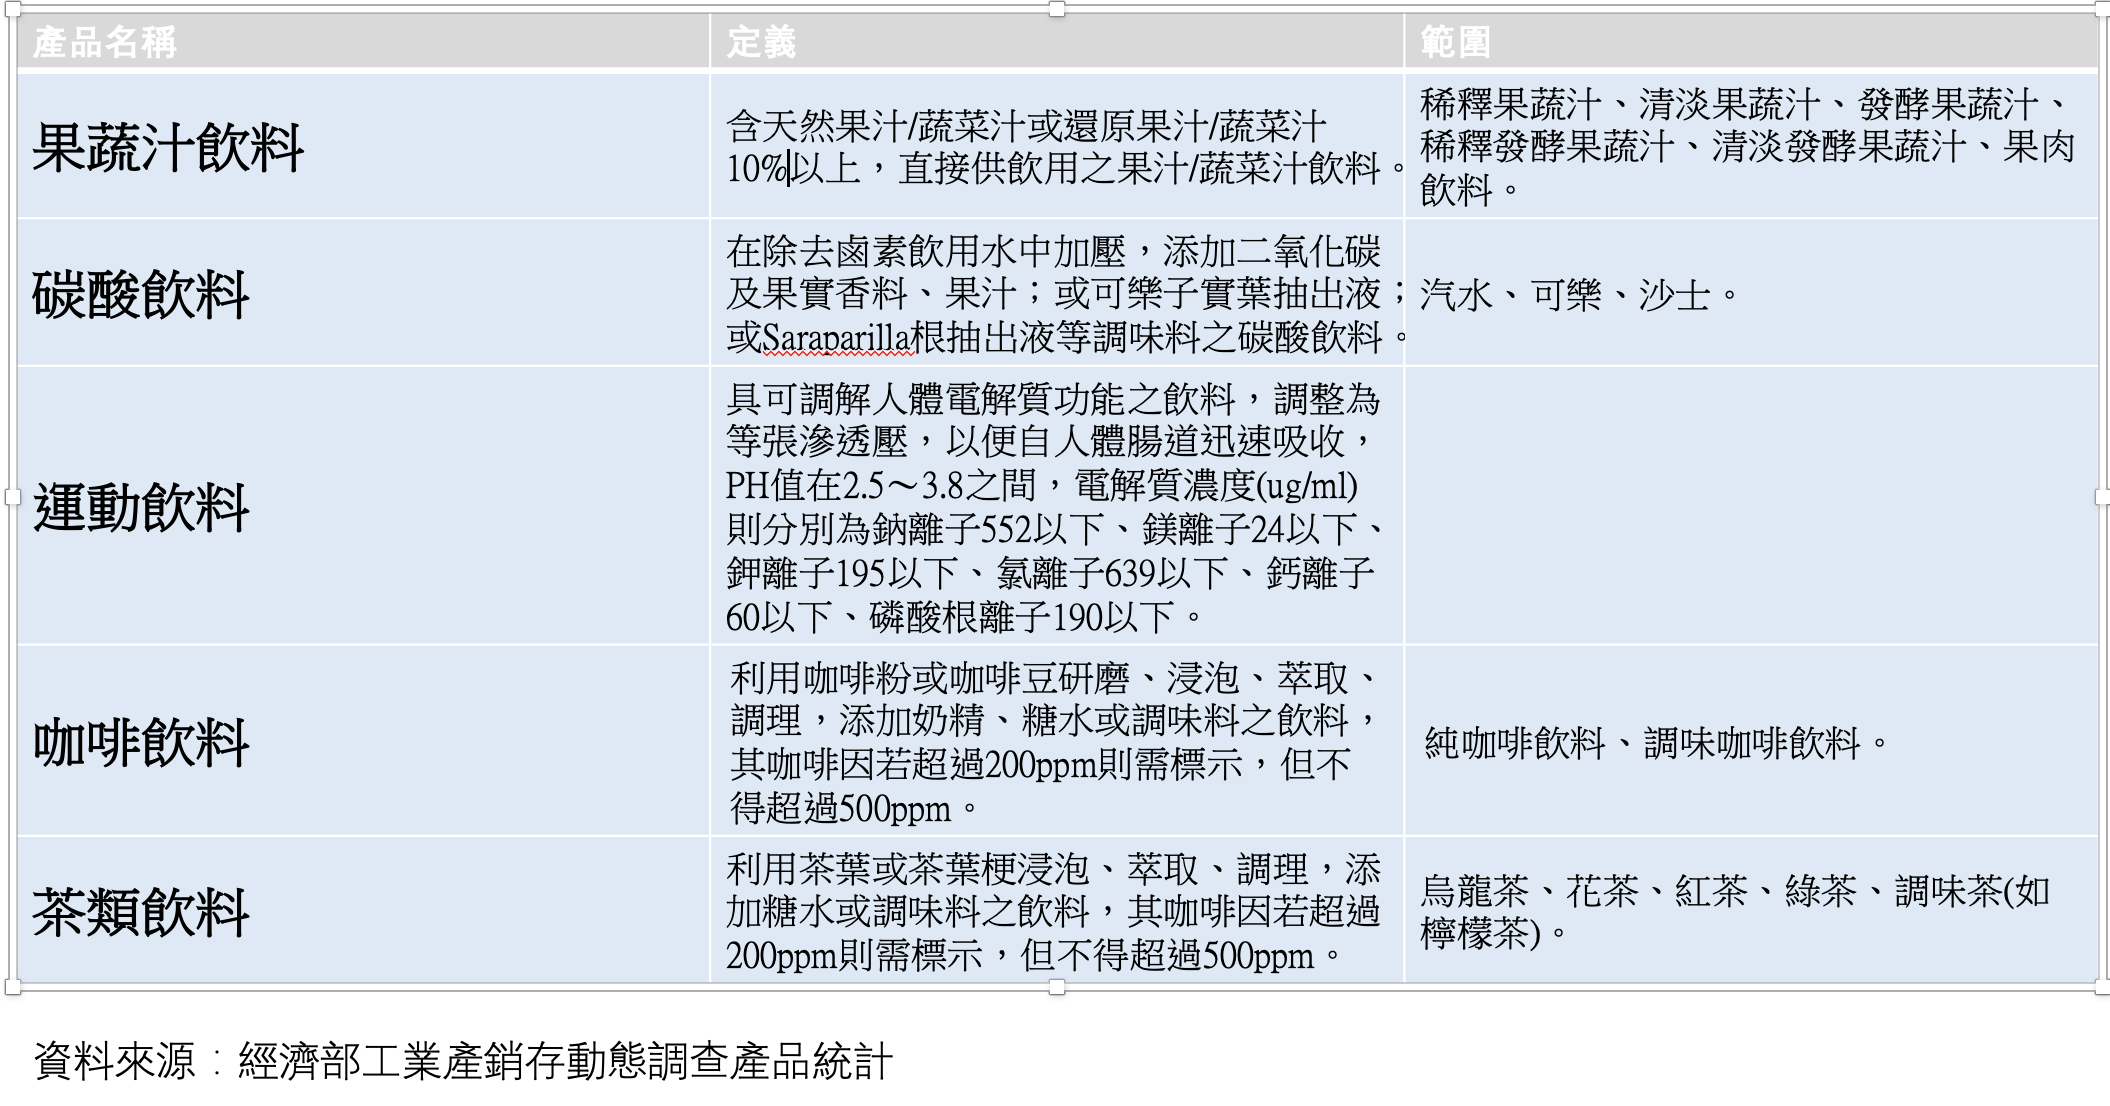
\includegraphics[width=1.0\textwidth]{figures/fig.png}
\end{frame}


\begin{frame}{Q4: What are the research questions raised in your DSE?}
	\begin{itemize}
		\item \textbf{消費者對不同飲料類別的價格彈性}:當價格變動時,消費者對果蔬汁飲料、碳酸飲料、運動飲料、咖啡飲料和茶類飲料的需求如何變化?是否某一類飲品對價格更敏感?
		\vspace{0.3cm}
		\item \textbf{不同飲料類別之間的交叉價格彈性}:當一類飲品的價格上升或下降時,是否會影響其他類似飲品的需求?
		\vspace{0.3cm}
		\item \textbf{收入水準變化對消費者飲料需求的影響}:隨著消費者收入的增長或減少,哪一類飲品的需求會受到最大影響?運動飲料、果蔬汁飲料或咖啡飲料是否更依賴於收入的變化?
	\end{itemize}
\end{frame}

\begin{frame}{Q5: Please provide sufficient background information about the topic you chose for your analyses.}
	\begin{itemize}
		\item \textbf{產品的市場覆蓋率和多樣性}:五類飲料涵蓋了當今飲料市場中最重要的細分市場,能夠代表大部分消費者的飲料需求,適合進行整體飲料市場的需求體系分析。
		\vspace{0.3cm}
		\item \textbf{消費行為差異}:些飲料類型反映了不同消費需求和偏好。例如,運動飲料主要消費於運動後恢復能量,而咖啡飲料更多與提神和日常工作需求相關。年輕人可能更偏好碳酸飲料和運動飲料,而中老年人則傾向於選擇果蔬汁和茶飲。
		\vspace{0.3cm}
		\item \textbf{健康意識的影響}:隨著健康意識的提升,果蔬汁和茶飲料逐漸受到追捧,而碳酸飲料面臨健康風險相關的負面影響。在 demand system 中加入這些不同健康屬性的飲料,可以更好地分析消費者健康意識對飲料選擇的影響。
		\vspace{0.3cm}
		\item \textbf{替代效應研究}:這五種類型的飲料之間存在替代關係,通過 demand system,可以分析不同飲料類型之間的影響,從而提供更全面的消費者市場需求預測。
	\end{itemize}
\end{frame}

% \begin{frame}{Data}{}
% 	\begin{itemize} 
		
		
		
% 		\item Our analysis is based on administrative data from the Health and Welfare Data Science
% 		Center (HWDC) in Taiwan
% 		\vspace{0.3cm}
% 		\item We use four sources of data hosted by HWDC for the main
% 		analysis
% 		\begin{itemize}
% 					\vspace{0.3cm}
% 			\item[1] The birth certificate registry, 
% 			\vspace{0.3cm}
% 			\item[2] Enrollment records of the National
% 			Health Insurance (NHI)
% 						\vspace{0.3cm}
% 			\item[3] The Catastrophic Illness Registry
% 									\vspace{0.3cm}
% 			\item[4] The outpatient medical utilization records
% 		\end{itemize}
	
		
% 	\end{itemize}
% \end{frame}



% \begin{frame}{Sample}{}
% 	\begin{itemize} 
		
		
		
% 		\item We created a balanced panel of
% 		parents whose first children were born between 2004 to 2007 
% 		\vspace{0.3cm}
% 		\item Follow them starting
% 		the 4th year before the birth of first-born and ending in the 10th after birth
% 		\begin{itemize}
% 			\vspace{0.3cm}
% 			\item The treatment group consists of parents whose first child is disabled
% 			\vspace{0.3cm}
% 			\item Restrict the disabilities were diagnosed
% 			under the age of three
% 			\vspace{0.3cm}
% 			\item The control group includes parents whose children
% 			did not have any catastrophic illnesses
% 		\end{itemize}
		
		
% 	\end{itemize}
% \end{frame}




% \begin{frame}{Empirical Specification}{Event-Study Design}
% 	\begin{eqnarray*}\label{dis_event}
% 	\hspace*{-3ex}    Y_{it} =  \nu_{i} + \lambda_{t} + a_{it} + \sum\limits^{10}_{\substack{k=-4\\k\neq-2}} \delta_{k} \mathbf{I}[t-E_{i}=k]  +  \varepsilon_{it},  
% 	\end{eqnarray*}
% 			\begin{itemize} 
% 		\item $Y_{it}$ represents an outcome of interest:
% 					\vspace{0.3cm}
% 		\begin{itemize} 
% 			\item Employment: a dummy indicating working at least one month or not	
% 			\vspace{0.3cm}
% 			\item Annual earnings
% 						\vspace{0.3cm}
% 		\end{itemize}	
% 	\item $E_{i}$ represents the year when individual $i$ has the first child with disability
% 							\vspace{0.3cm}
% 	\item $\mathbf{I}[t-E_{i}=k]$ is an indicator for being $k$ years from the birth of a disabled child
% 			\vspace{0.3cm}
% 	\item $\delta_{k}$ represent the difference in labor supply outcomes between the treatment and the control groups in the $k^{th}$ year relative to baseline gap
	
% 			\begin{itemize} 
% 							\vspace{0.3cm}	
		
% 		\item We use \(k=-2 \) as the baseline year such that the coefficient \(\delta_{-2} \) is normalized to zero	
% 						\end{itemize}	
				
% 	\end{itemize}
% \end{frame}



% \begin{frame}{Trend in Employment Rate between Treatment and Control Group}{Female}
% 	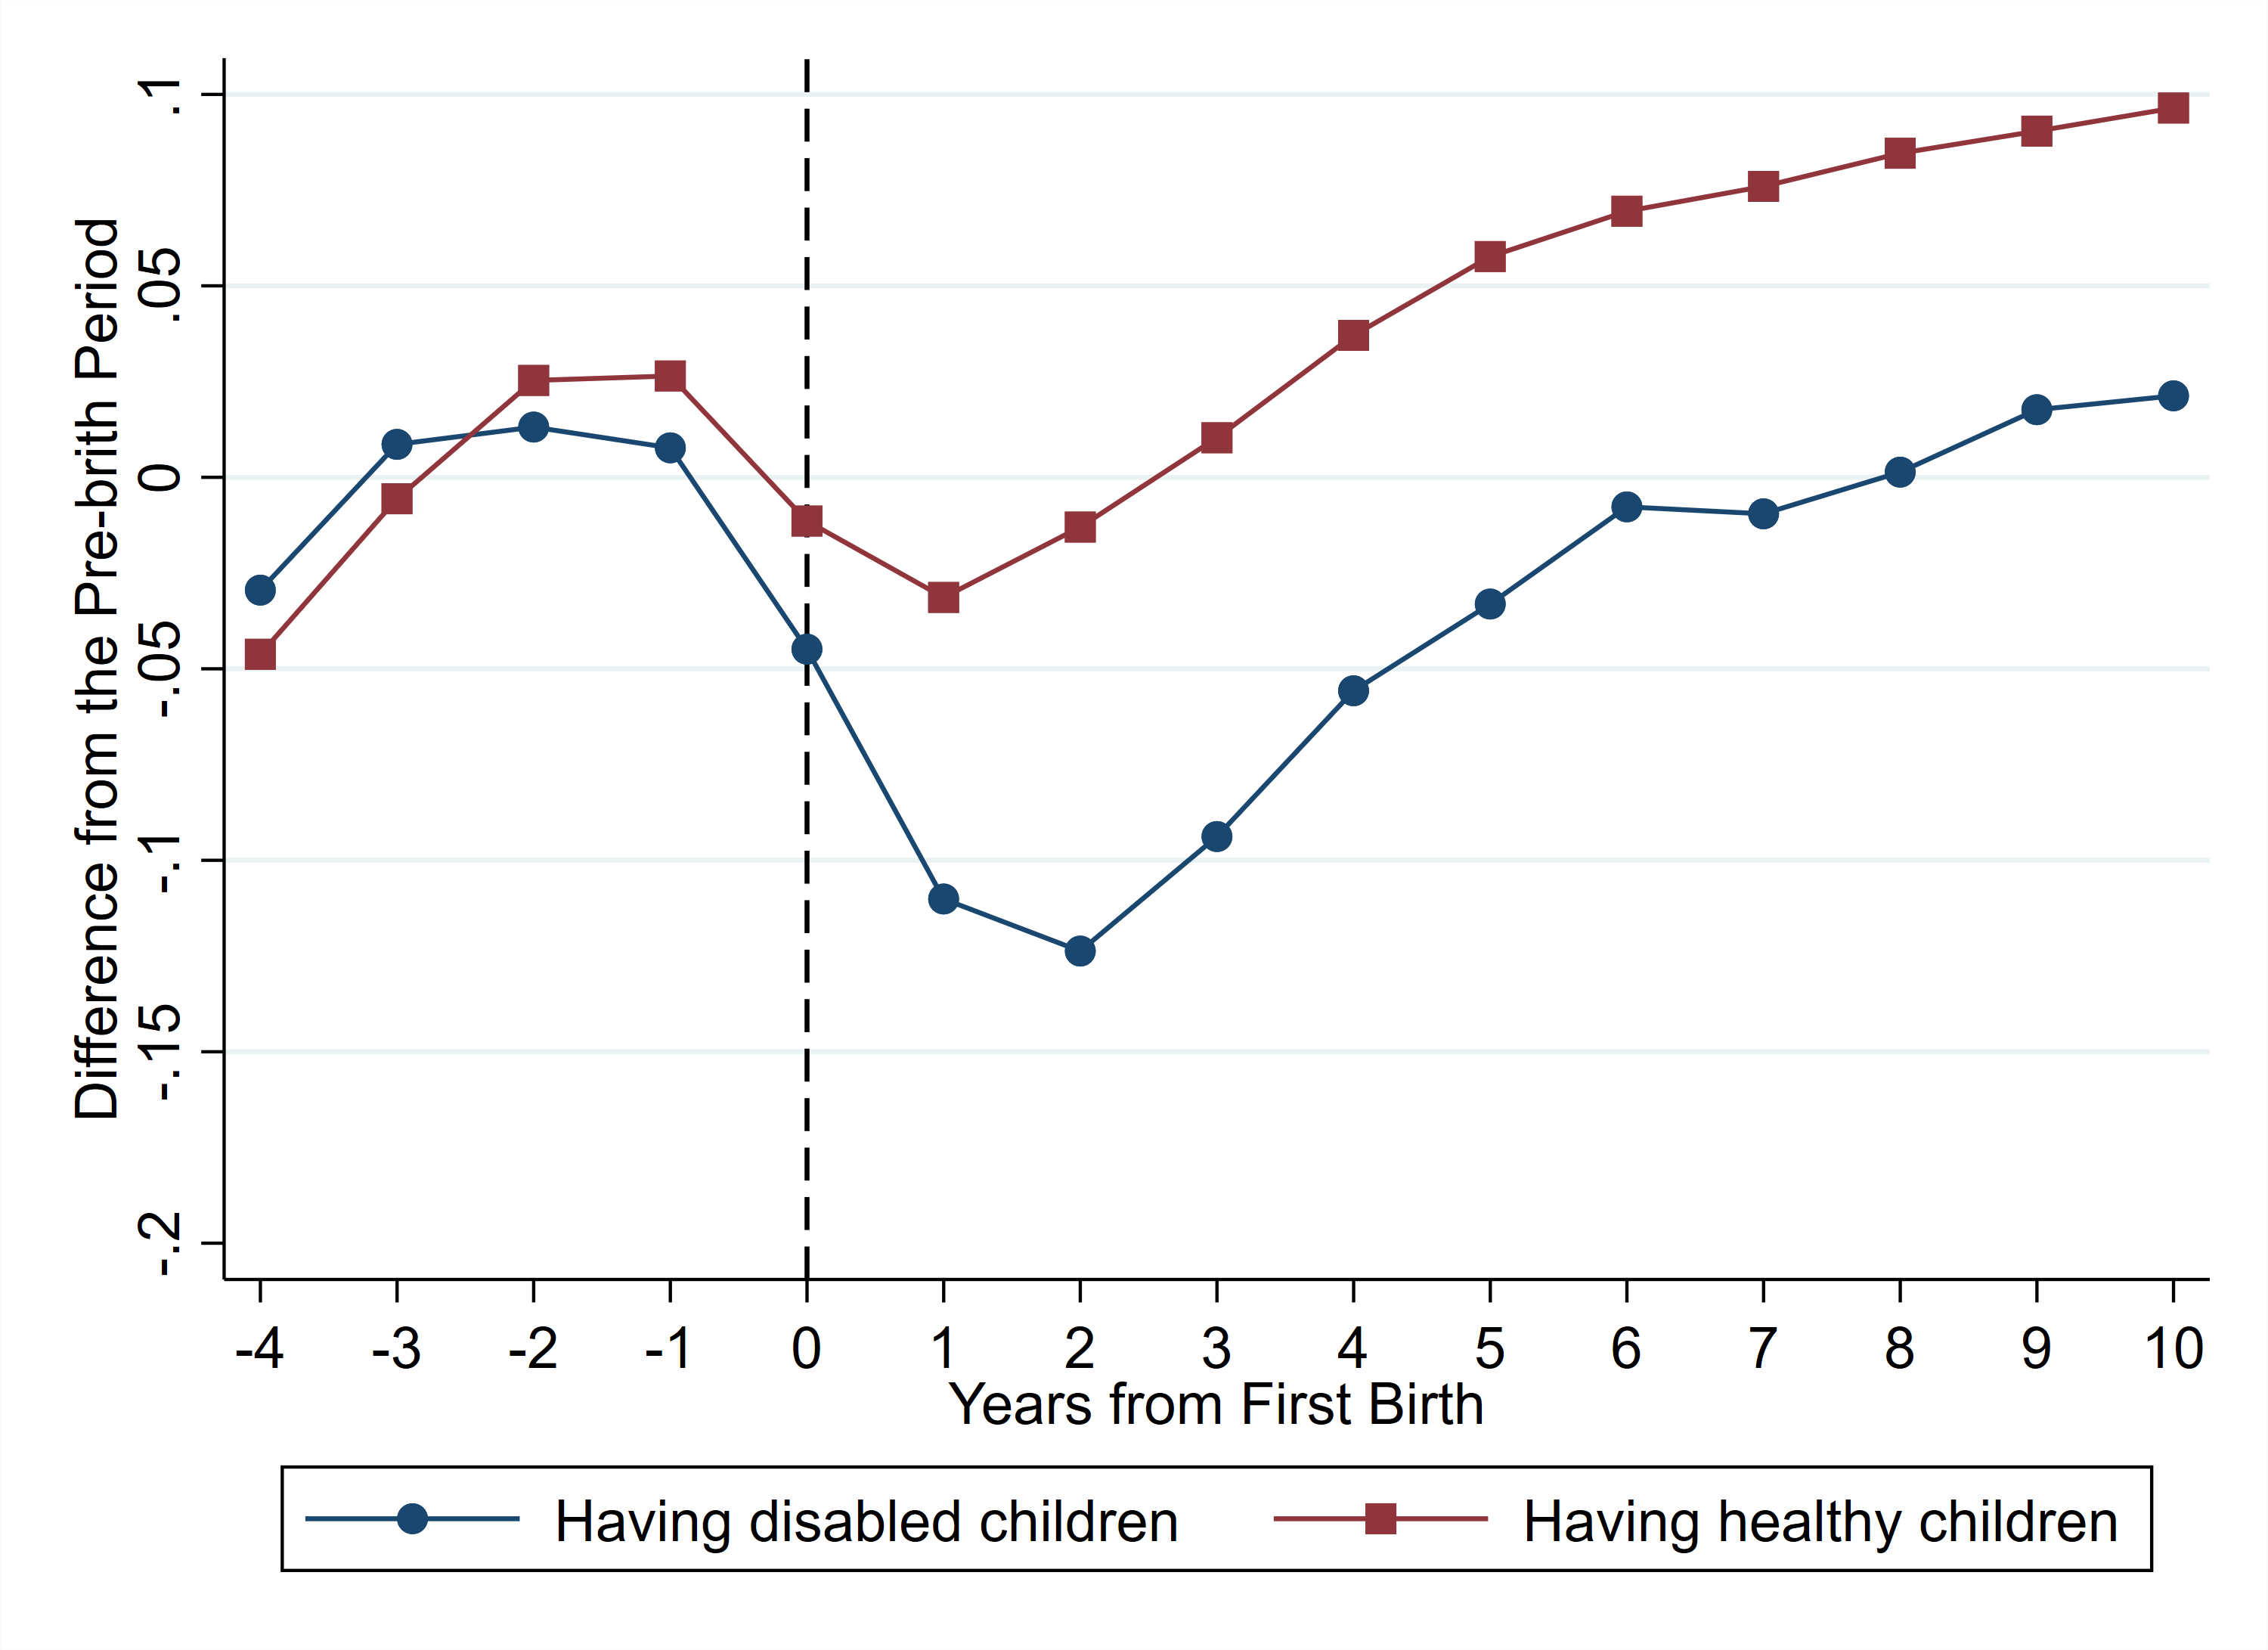
\includegraphics[width=1.0\textwidth]{figures/Figure_1_work_least_perc_perm_female.png}
	
% \end{frame}



% % \begin{frame}{Empirical results: Constructing treatment status}
% % \begin{table}[H]
% % \centering
% % \begin{tabular*}{\textwidth}{@{\extracolsep{\fill}}l*{4}{S[table-format=2.1]}}
% %     \Xhline{1pt}
% %      & {\multirow{2}{*}{Control}} & \multicolumn{3}{c}{Treated} \\
% %      \cmidrule
% %      & & {All} & {Repeal} & {Decrease} \\
% %     \Xhline{0.8pt}
% %     Log net estate & 14.9 & 16.2 & 15.8 & 16.6 \\
% %     Age & 74.3 & 75.3 & 75.1 & 75.4  \\
% %     Num of kids &  3.5 & 3.6 & 3.5 & 3.7 \\
% %     Male (share) &  68 & 69 & 66 & 72 \\
% %     Married (share) &  52 & 53 & 47 & 58 \\
% %     \addlinespace[1ex]
% %     Num of observations &  99,891 &  45,838 & 20,701 & 25,137 \\
% %     \Xhline{1pt}
% % \end{tabular*}
% % \end{table}
% % \end{frame}


% \begin{frame}{Results: DiD by treated group}

%  \begin{table}[]
%     \centering
%     \begin{tabular}{lcccc}
%     \hline
%     Treated is & & All & Repeal & Decrease \\
%       & & (1) & (2) & (3) \\
%     \hline
%     \textbf{Panel A: Log net estate} \\
%     Treated $\times$ Post & & 0.099 & 0.116 & 0.133 \\
%     & & (0.013) & (0.014) & (0.016)  \\  
%     \hline
%     Treated N & & 45,838 & 20,721 & 25,137 \\
%     \hline
%     \end{tabular}
% \end{table}
% \end{frame}

\end{document}
